\documentclass[../main.tex]{subfiles}
\begin{document}
\subsubsection{Linear ODEs}\label{subsubsec1.2.0}
\paragraph{Inhomogeneous}
We will consider the linear case first with non-constant forcing.
\begin{theorem}[label=thm1.2.1]{}{}
     Let $f,g$ be two continuous functions, then the ODE
     \begin{equation*}
          \newprime{y}(x) + f(x)y(x) = g(x)\,,
     \end{equation*}
     has a general solution
     \begin{equation*}
          y(x) = \frac{C + \int_{}^{}e^{\int_{}^{}f(x)dx}g(x)dx}{e^{\int_{}^{}f(x)dx}} \,. 
     \end{equation*}
\end{theorem}
\begin{proof}
     Suppose there exist $h(x)$ (often called the \textbf{integrating factor}) s.t. $\newprime{h}(x)=h(x)f(x)$. 
     We can multiply both sides of the ODE by such function to get
     \begin{equation*}
             g(x)h(x) = \newprime{y}(x)h(x)+\underbrace{h(x)f(x)}_{\newprime{h}(x)}y(x) = \underbrace{\newprime{y}(x)h(x)+\newprime{h}(x)y(x)}_{\text{product rule}} = \newprime{(y(x)h(x))}\,.
     \end{equation*}
Integrating both sides gives
\begin{equation*}
        \int_{}^{}\newprime{(y(x)h(x))}dx = y(x)h(x) + C_{1} = \int_{}^{}g(x)h(x)dx\quad\Rightarrow\quad y(x) = \frac{\int_{}^{}g(x)h(x)dx - C_{1}}{h(x)}\,.
\end{equation*}
Now in order to get an explicit form for $h(x)$ we use the initial requirement for its definition to get
\begin{equation*}
     \newprime{h}(x)=h(x)f(x) \quad\Rightarrow\quad f(x)=\frac{\newprime{h}(x)}{h(x)}=\newprime{(\log(h(x)))}\,.
\end{equation*}
Integrating both sides yields
\begin{equation*}
\int_{}^{}f(x)dx=\int_{}^{}\newprime{(\log(h(x)))}dx = \log(h(x)) + C_{2}\quad\Rightarrow\quad h(x) = \underbrace{e^{\;-C_{2}}}_{C_{3}}{}^{+\int_{}^{}f(x)dx} = C_{3}\,e^{\int_{}^{}f(x)dx}\,.
\end{equation*}
Plugging this expression into the above form for the solution concludes the proof
\begin{equation*}
        y(x) = \frac{\int_{}^{}C_{3}\,e^{\int_{}^{}f(x)dx}g(x)dx-C_{1}}{C_{3}\,e^{\int_{}^{}f(x)g(x)dx}} = \frac{C+\int_{}^{}\,e^{\int_{}^{}f(x)dx}g(x)dx}{e^{\int_{}^{}f(x)g(x)dx}}\,,\quad C:=-\frac{C_{1}}{C_{3}}\,.
\end{equation*}
\end{proof}
\begin{interpretation*}{}
     The solution strategy for linear, first-order ODEs goes as follows:
     \begin{enumerate}
          \item put the ODE in standard form (i.e. compute $f$ and $g$);
          \item compute the integrating factor $h$;
          \item multiply both sides of the ODE by $h$ and simplify the product rule on the LHS;
          \item integrate both sides and use the FTC to isolate the solution $y$ in terms of $h$ and $g$;
          \item determine the integration constant $C$ using the BCs.
     \end{enumerate}
\end{interpretation*}
\begin{example}[label=ex1.2.0.0]{}{}
     Let us consider the following Cauchy IVP
     \begin{equation*}
        \begin{cases}
            x \newprime{y} + 3y = 4x^{2}-3x\,, \quad x\in(0,1]\\
            y(1) = 0\,, 
        \end{cases}
     \end{equation*}
     we now follow the steps of the solution strategy introduced above to find a general integral (or family of solutions) of the ODE and a particular solution for the IVP:
\end{example}
\begin{example_continued}
     \begin{enumerate}
          \item we put the ODE in standard form by diving both sides by $x$
                  \begin{equation*}
                          \newprime{y} + \underbrace{\frac{3}{x}}_{f(x)}y = \underbrace{4x - 3}_{g(x)}\,;
                  \end{equation*}
          \item we compute the integrating factor
                  \begin{equation*}
                       h(x) = e^{\int_{}^{}f(x)dx} = e^{\int_{}^{}\frac{3}{x}dx} = e^{3\ln x} = e^{\ln x^{3}} = x^{3}\,;
                  \end{equation*}
          \item we multiply both sides of the ODE in step $1.$ by the integrating factor and simplify the product rule
                  \begin{equation*}
                       x^{3}\newprime{y}+3x^{2}y = \newprime{(x^{3}y)} = 4x^{4} - 3x^{3}\,;
                  \end{equation*}
          \item we integrate both sides of the ODE above 
                  \begin{equation*}
                       \int_{}^{}\newprime{(x^{3}y)}dx = x^{3}y + C_{1} = \int_{}^{}4x^{4}dx - \int_{}^{}3x^{3}dx = \frac{4}{5}x^{5} + C_{2} - \frac{3}{4}x^{4} + C_{3}\,,
                  \end{equation*}
                  and isolate $y$ on the LHS
                  \begin{equation*}
                       y = \frac{4}{5}x^{2} - \frac{3}{4}x + \frac{C}{x^{3}}\,,\quad C:=C_{2}+C_{3}-C_{1}\,,
                  \end{equation*}
                  which is now our family of solutions of the ODE parametrised by $C$;
          \item we impose the BC $y(1)=0$ to determine the value of $C$ and extract the unique solution that satisfy the IVP 
                  \begin{equation*}
                       0 = \frac{4}{5} - \frac{3}{4} + C \; \Rightarrow \; C = \frac{3}{4} - \frac{4}{5} = -\frac{1}{20}\,, 
                  \end{equation*}
                which gives us the curve
                  \begin{equation*}
                       y(x) =  \frac{4}{5}x^{2} - \frac{3}{4}x - \frac{1}{20}x^{-3}\,.
                  \end{equation*}
     \end{enumerate} 
\end{example_continued}
\begin{example_continued}
     \begin{figure}[H]
         \centering 
         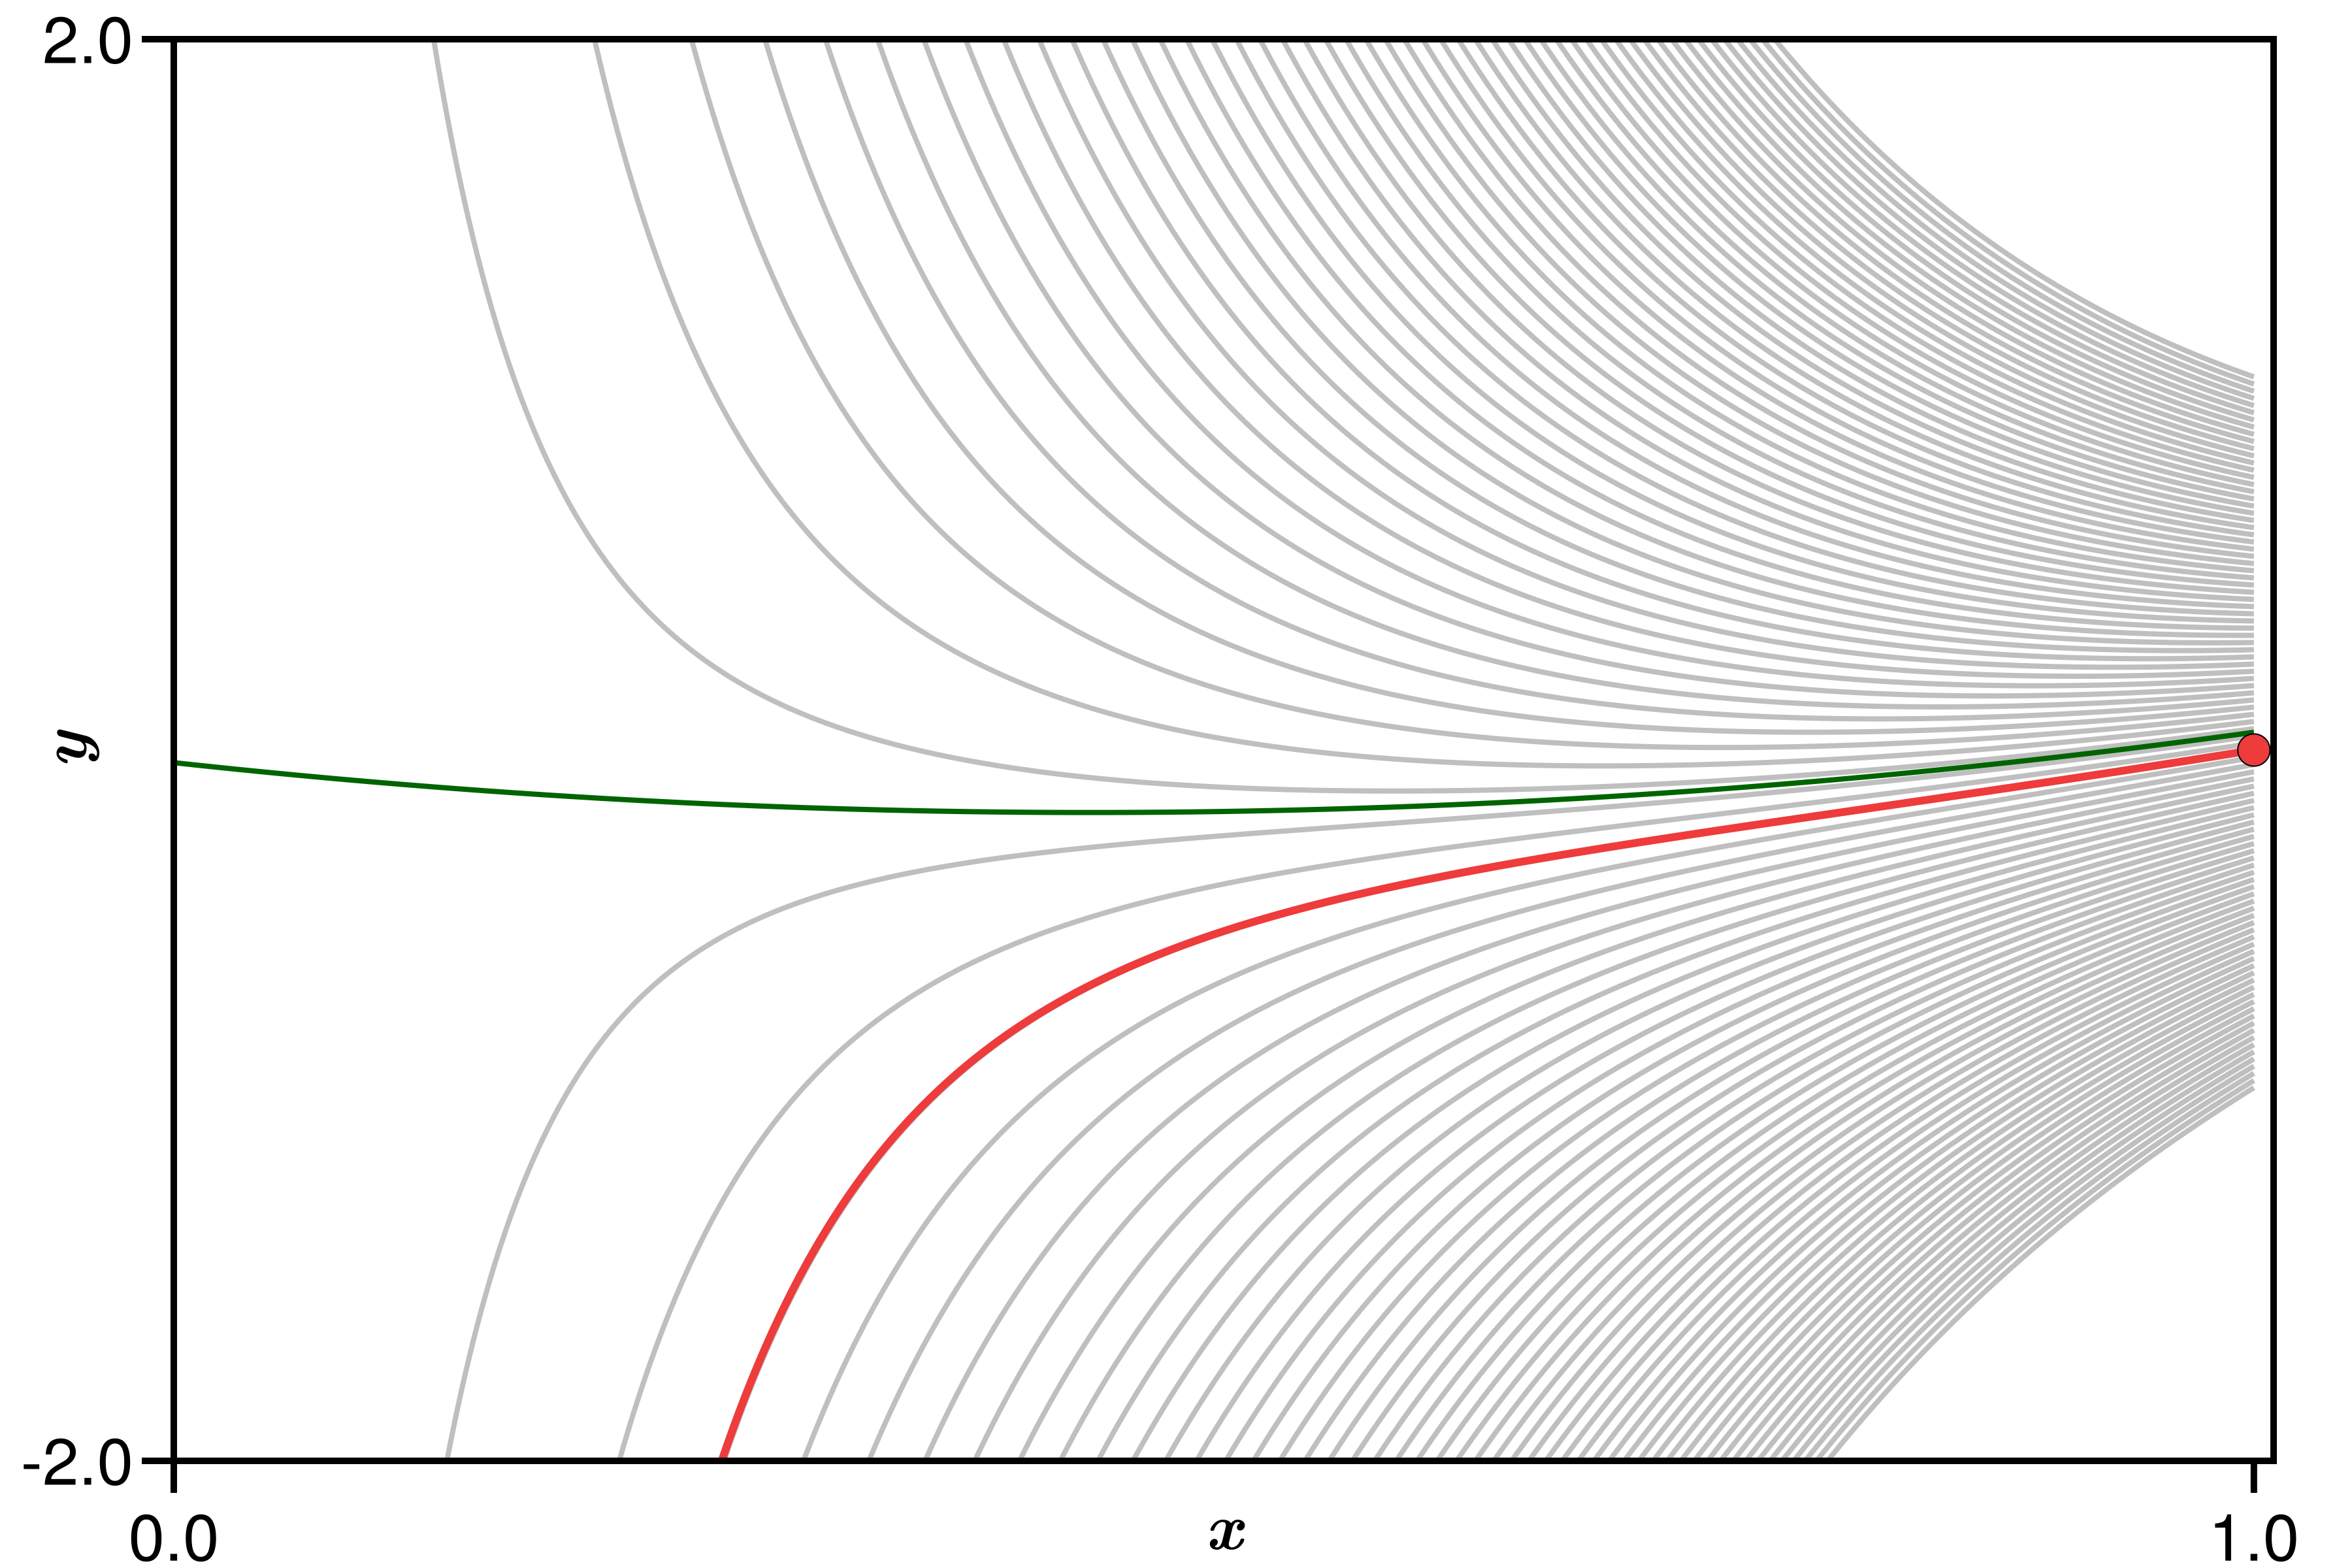
\includegraphics[keepaspectratio, width=0.75\textwidth]{../figures/figure1.2.0.0.png}
         \caption{Family of solutions (gray lines) of the linear ODE in $(0,1]$ at different values of the integration constant $C\in[-1,1]$ and the solution of the IVP (red line) for the constant value $C=-\frac{1}{20}$ satisfying the BC $y(1)=0$ (red dot).
         Note that the only bounded solution (green curve) is at $C=0$.}
         \label{fig1.2.0.0}
     \end{figure}
\end{example_continued}
\begin{example}[label=ex1.2.0.1]{}{}
     We repeat the same procedure to the find the solution of the following Cauchy IVP
     \begin{equation*}
        \begin{cases}
            (x-2)\newprime{y} + y = 3x^{2} +2x \,, \quad x\in[-1,1]\\
            y(1) = -1\,: 
        \end{cases}
     \end{equation*}
\end{example}
\begin{example_continued}
    \begin{enumerate}
            \item ;
            \item ;
            \item ;
            \item $y=\frac{x^{3}+x^{2}+C}{x-2}$;
            \item $C = -1$;
    \end{enumerate} 
\end{example_continued}
\begin{example_continued}
     \begin{figure}[H]
         \centering 
         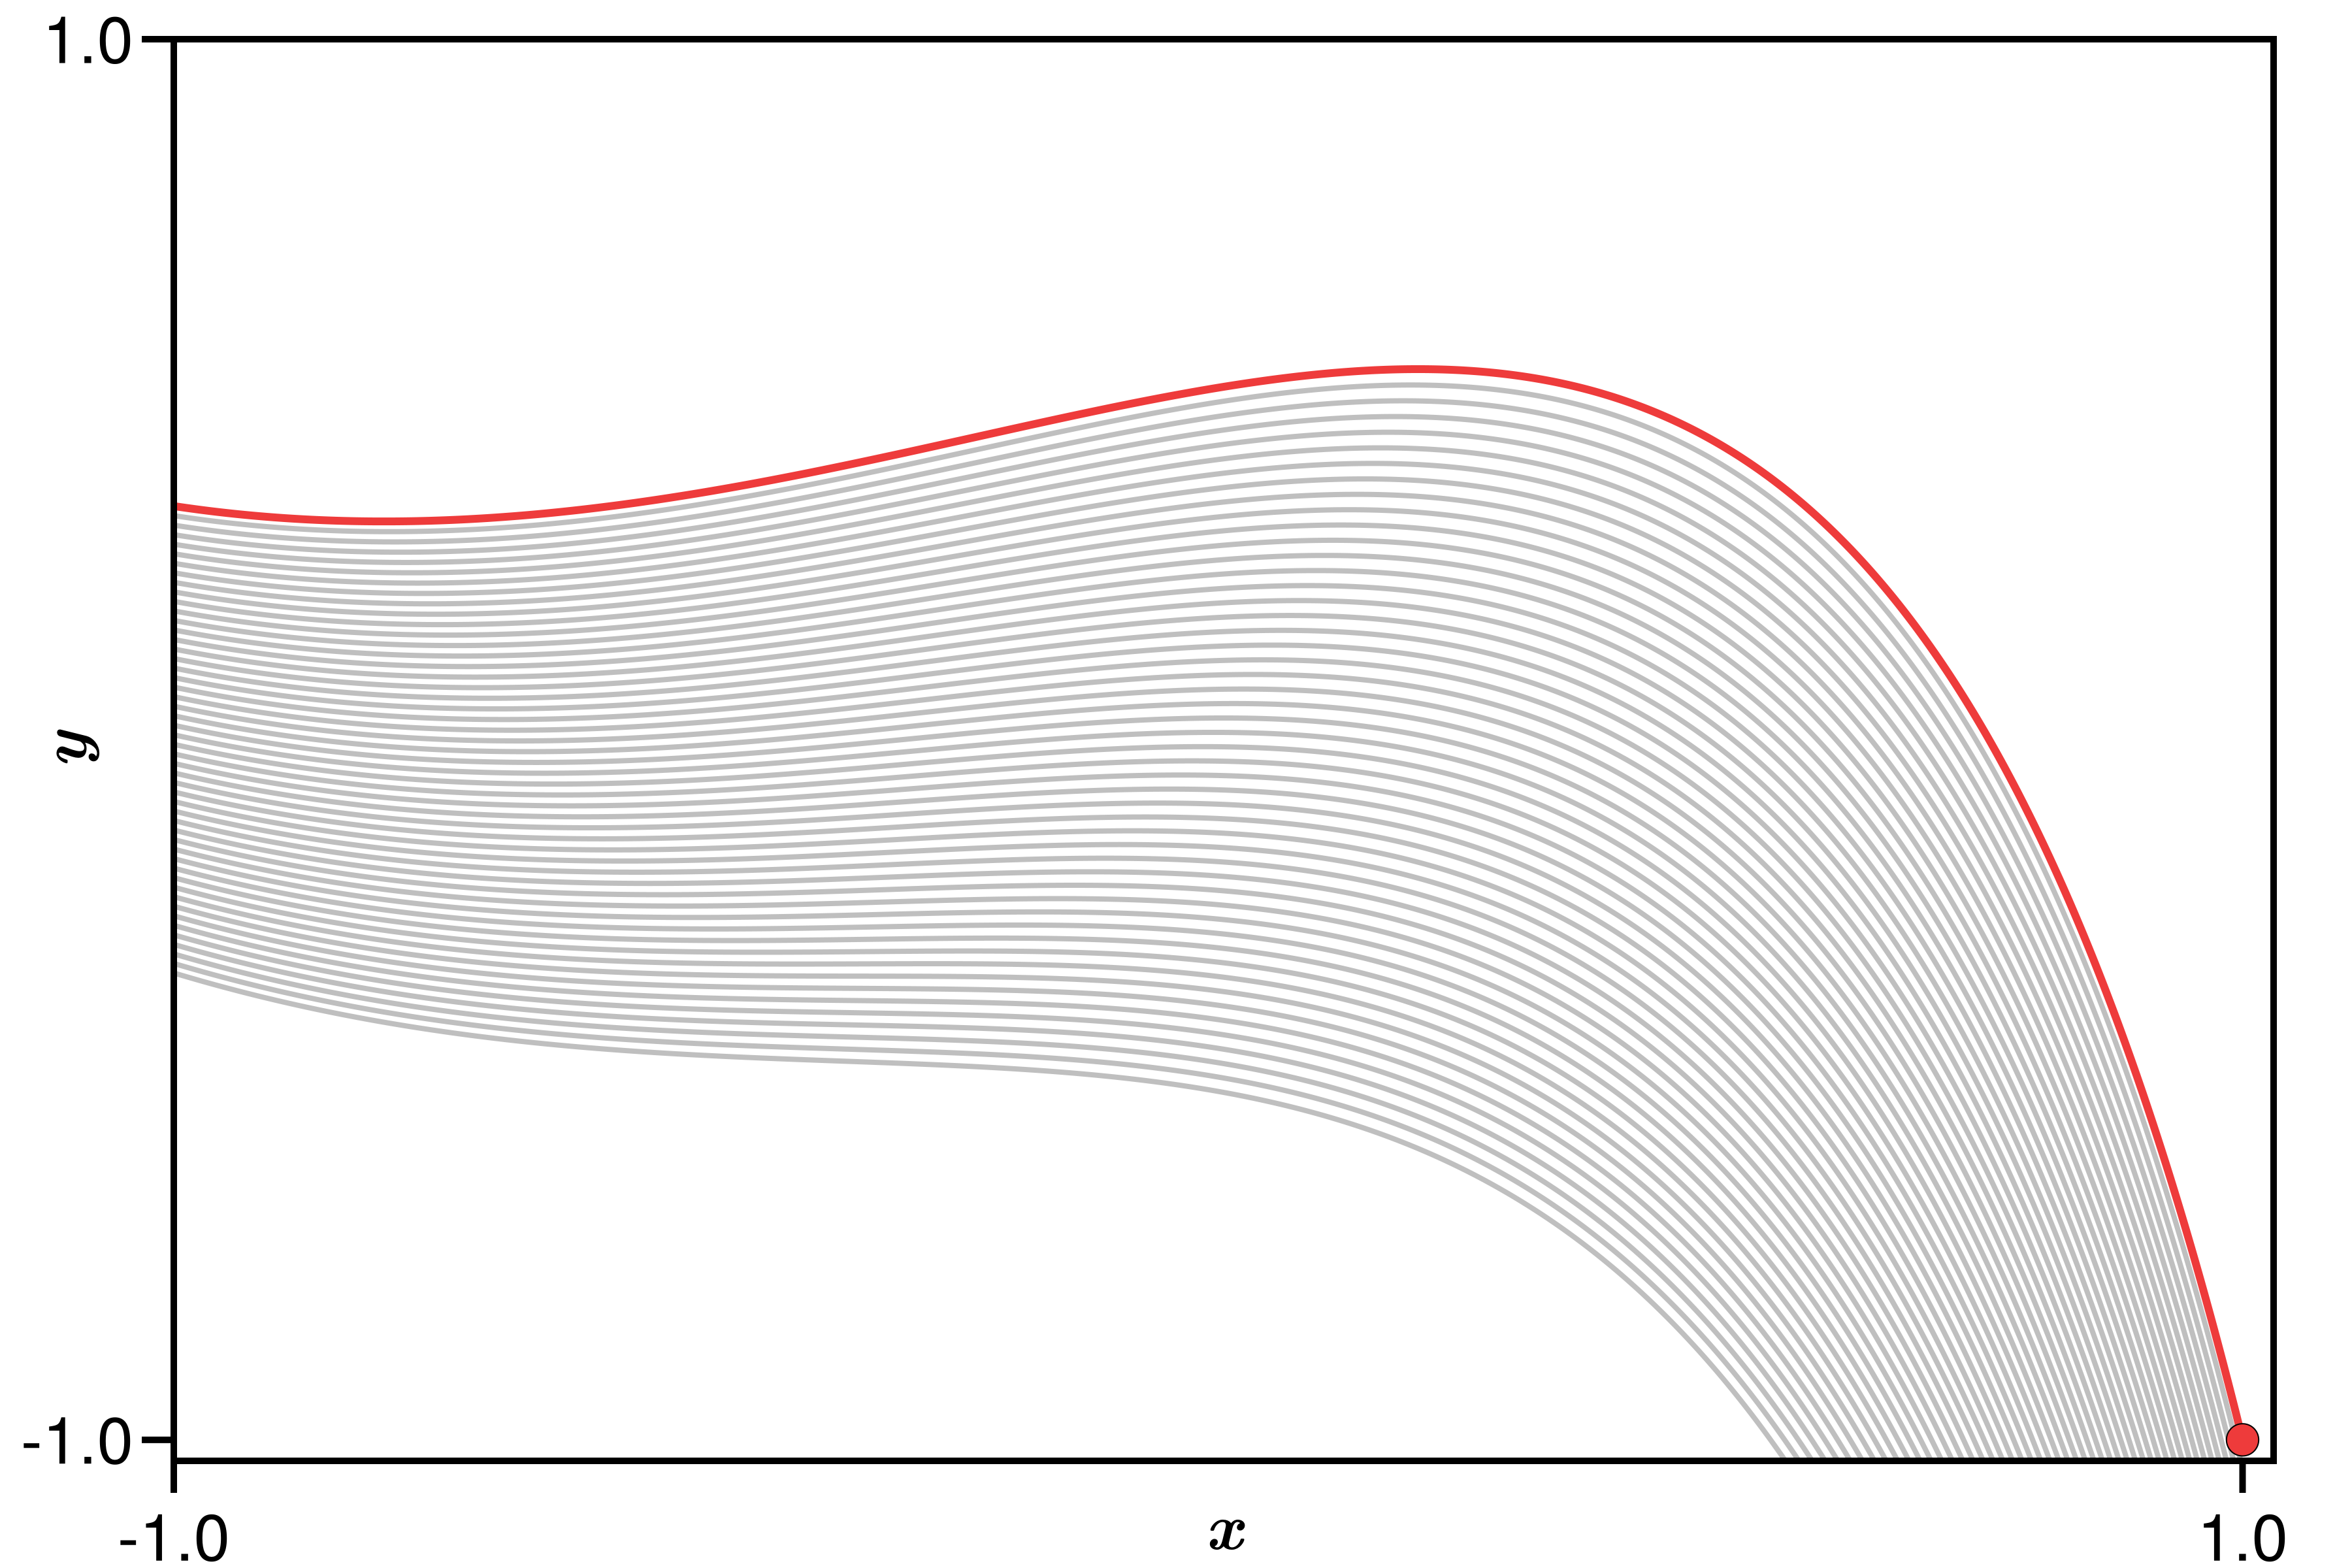
\includegraphics[keepaspectratio, width=0.75\textwidth]{../figures/figure1.2.0.1.png}
         \caption{Family of solutions (gray lines) of the linear ODE in $[-1,1]$ at different values of the integration constant $C\in[-1,1]$ and the solution of the IVP (red line) for the constant value $C=-1$ satisfying the BC $y(1)=-1$ (red dot).}
         \label{fig1.2.0.1}
     \end{figure}
     
\end{example_continued}
\end{document}
